\documentclass[../rapporto-usabilita.tex]{subfiles}

\begin{document}
\section{Risultati dell'analisi}
	\subsection{Analisi generale}
	\label{sec:analisigenerale}
	
	Di seguito sono riportati i risultati dell'analisi sull'usabilità del sito nel suo complesso. Le osservazioni seguenti sono valide per tutte le pagine del sito, si è deciso quindi di raccoglierle in una sezione unica per evitare ripetizioni.
	
		\subsubsection{Gli assi principali}
			
			\begin{figure}[!h]
			\centering
				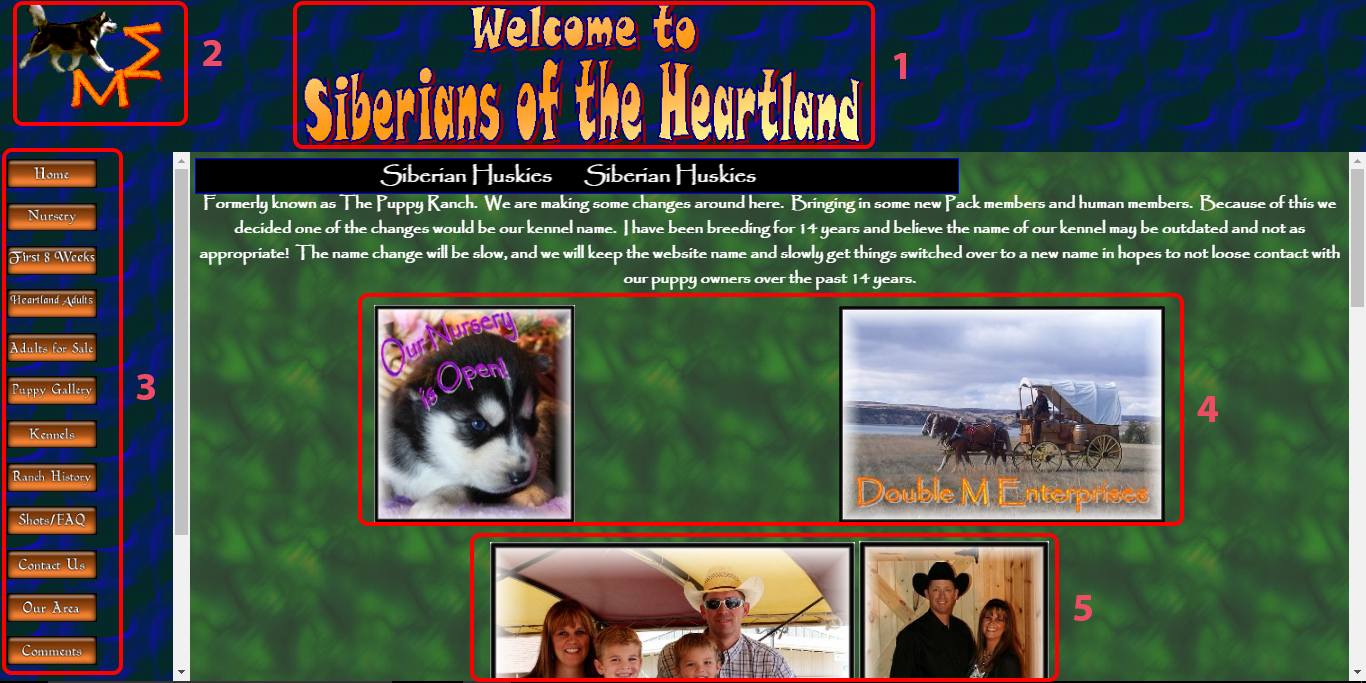
\includegraphics[scale=0.33]{immagini/home_focus.jpg}
				\caption{La prima parte della pagina \textit{Home}.}
				\label{fig:homefocus}
			\end{figure}	
		
			\paragraph{Where}
				Il nome del sito è riportato nella parte alta della pagina ed è quindi immediatamente visibile (\hyperref[fig:homefocus]{Figura 1.1}) . \textbf{Positivo}. Si nota, però, come il nome del sito (\textit{Siberians of the Heartland}) sia completamente diverso dal nome del dominio (\textit{thepuppyranch.com}). Questo richiede un maggiore sforzo mnemonico all'utente che voglia raggiungere il sito direttamente o che non riesca a trovarlo tramite motore di ricerca.
				
			\paragraph{Who}
				Il logo dell'azienda rappresentata dal sito è riportato in alto a sinistra (\hyperref[fig:homefocus]{Figura 1.2}), la sezione "Ranch History" presenta brevemente l'azienda ed i suoi fondatori. \textbf{Positivo}.
				
			\paragraph{Why}
			 	Riportare uno slogan e/o prevedere una sezione che spieghi i punti di forza dell'azienda è utile per convinvere l'utente a scegliere questo sito piuttosto che un concorrente.
			 	In questo caso non è previsto nulla di tutto ciò. \textbf{Negativo}. 
				
			\paragraph{When}
				Si veda la sezione \hyperref[sec:analisiparti]{Analisi delle parti}. 
				
			\paragraph{What}
				Non esiste una sezione dedicata a spiegare di cosa si occupi l'azienda rappresentata dal sito.
				Ad una prima visita non è semplice capire che l'azienda rappresentata dal sito si occupa di allevare e vendere cuccioli.				
				 Una breve descrizione viene fornita nella pagina \textit{Home} ma, per raggiungerla, sono necessari 3 scroll. L'utente medio difficilmente si spinge oltre i 2 scroll, quindi un contenuto posto a 3 scroll di distanza è praticamente invisibile. \textbf{Negativo}. 
			
			\paragraph{How}
				Nella parte sinistra del sito è presente un menù di navigazione che permette all'utente di raggiungere tutte le sezioni principali del sito (\hyperref[fig:homefocus]{Figura 1.3}). \textbf{Positivo}.
		
		\subsubsection{Inconsistenza dei frame}
		
			\begin{figure}[!h]
			\centering
				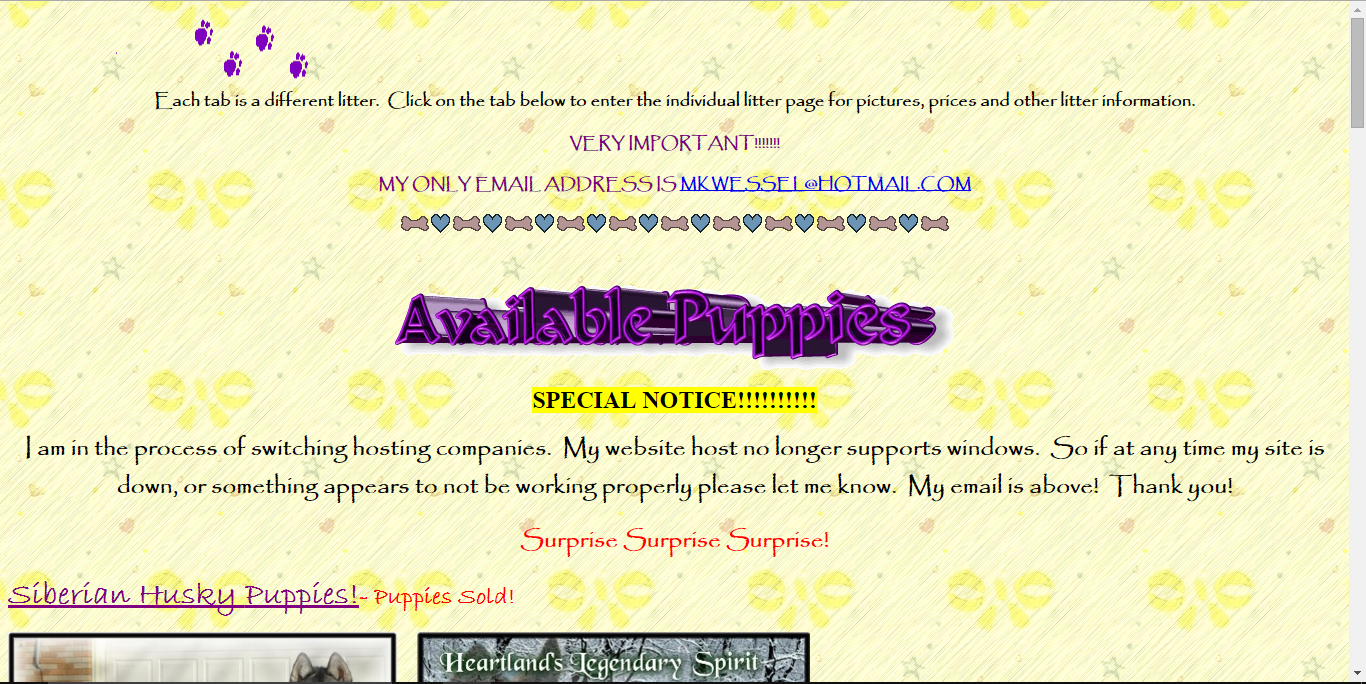
\includegraphics[scale=0.33]{immagini/nursery.png}
				\caption{Una pagina interna acceduta direttamente dalla SERP.}
				\label{fig:innerpage}
			\end{figure}			
		
		La struttura del sito è costruita attraverso l'utilizzo di frame, in particolare sono utilizzati tre frame:
		
		\begin{itemize}
			\item \textit{Banner}: ospita il logo ed il nome del sito;
			
			\item \textit{Content}: ospita il menù di navigazione;
			
			\item \textit{Main}: ospita il contenuto della sezione corrente del sito.
		\end{itemize}
		
		Ogni frame contiene una diversa pagina web e queste vengono combinate tra loro per ottenere un classico layout a tre pannelli.
		Quando si seleziona una voce del menù o si apre un link verso una pagina interna, la nuova pagina viene aperta all'interno del frame \textit{Main}.
	Questro approccio presenta un problema fondamentale: se le pagine interne del sito vengono indicizzate da un motore di ricerca, l'utente può raggiungere una pagina interna direttamente dalla SERP senza passare dalla pagina \textit{Home}. Questo provoca la perdita della struttura a frame e l'utente visualizza solamente la pagina interna, ovvero il \textit{Main}. In questo modo l'utente perde i riferimenti agli assi \textit{Who} ed \textit{How} (\hyperref[fig:innerpage]{Figura 2}). \textbf{Negativo}.
	
		\subsubsection{Lost in navigation}
			Le pagine del sito sono sprovviste di \textit{breadcrumb}, inoltre i link vengono tutti presentati sotto forma di immagini e non viene adottata alcuna convenzione per indicare quelli già visitati. Questo può infastidire l'utente, in quanto non riesce a capire facilmente in quale sezione del sito si trovi e quali sezioni abbia già visitato. \textbf{Negativo}.
			
		\subsubsection{Profondità}
		Il sito ha una struttura poco profonda ed ogni informazione disponibile può essere raggiunta in meno di tre click.  \textbf{Positivo}.
			
		\subsubsection{Scrolling}			
		
			\begin{figure}[!h]
			\centering
				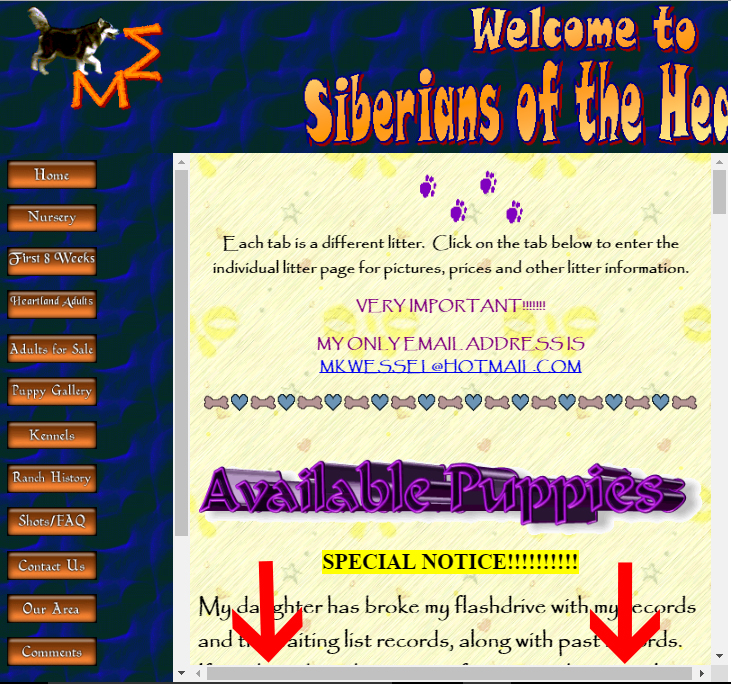
\includegraphics[scale=0.33]{immagini/horizontal_scroll.jpg}
				\caption{Una pagina con scroll orizzontale.}
				\label{fig:horizontalscroll}
			\end{figure}					
		
		Ogni frame si comporta come una pagina a se stante; questo significa che se il frame è troppo grande per lo schermo sul quale viene visualizzato, verrà automaticamente dotato di \textit{scrollbar} verticale e/o orizzontale.
		
			In particolare, il sito necessita di scroll orizzontale se lo schermo sul quale viene visualizzato ha larghezza minore di 810 px (\hyperref[fig:horizontalscroll]{Figura 3}). Lo scroll orizzontale è da evitare assolutamente in quanto aumenta di molto lo sforzo computazionale richiesto all'utente. 
		
		Il menù di navigazione è dotato di una propria \textit{scrollbar} verticale. Una \textit{scrollbar} dedicata al menù di navigazione (ed, in generale, qualsiasi \textit{scrollbar} diversa da quella principale) è inusuale e può creare confusione. Inoltre una tale disposizione nasconde all'utente inesperto le ultime voci del menù. \textbf{Negativo}.
		
		\subsubsection{Back button}
		Il \textit{back button} risulta abilitato e funzionante in 		tutte le pagine. Questo riduce lo sforzo computazionale dell'utente. \textbf{Positivo}. 
	
		\subsubsection{Apertura link}
		I link vengono aperti nella finestra corrente del browser, nessuna nuova finestra viene aperta automaticamente. Questo contribuisce a mantenere coerente l'effetto del back button. \textbf{Positivo}.
	 
	 	\subsubsection{Splash page}
	 	Non è presente la \textit{splash page} e non è richiesta alcuna registrazione per proseguire la navigazione sul sito. Questo evita all'utente inutili perdite di tempo. \textbf{Positivo}.
	 	
	 	\subsubsection{Convenzioni non rispettate}
	 	Rispettare le convenzioni adottate dalla maggioranza del web diminuisce lo sforzo computazionale richiesto all'utente per comprendere ed utilizzare il sito.
	 	
	 	\begin{itemize}
	 		\item Il logo va posizionato in alto a sinistra. \textbf{Rispettato};
	 		
	 		\item Solo le parti di testo che corrispondono a dei link vanno sottolineate e/o colorate in modo diverso dal resto del testo. \textbf{Non rispettato}. Si veda \hyperref[sec:analisiparti]{Analisi delle parti} per esempi specifici;
	 		
	 		\item I bottoni devono essere cliccabili. \textbf{Non rispettato}. La voce "Comments" del menù di navigazione non è cliccabile.
	 	\end{itemize}
	 
	 	\subsubsection{Bloated design}
	 	
			\begin{itemize}
	 		\item Non sono presenti fonti audio che possano arrecare fastidio all'utente \textbf{Positivo};
	 		
	 		\item L'installazione di plugin non è necessaria per usufruire del sito e non viene mai richiesta. \textbf{Positivo};
	 		
	 		\item Non sono presenti video che appesantiscono la banda necessaria lato server. \textbf{Positivo};
	 		
	 		\item Il logo del sito è un'immagine animata, questo può risultare fastidioso agli occhi dell'utente. \textbf{Negativo};
	 		
	 		\item Non è fornito un facile accesso al \textit{resize} del testo. \textbf{Negativo};
	 		
	 		\item I font usati risultano poco leggibili in quanto molto diversi dal classico Verdana al quale è abituato l'utente medio del web. Questo aumenta lo sforzo necessario alla lettura. \textbf{Negativo}.
	 	
	 	\end{itemize}
	 	
	 \subsubsection{Versione \textit{mobile}}
	 
	 	Circa il 40\% degli utenti che possiedono uno smartphone lo usa per accedere al web in mobilità e, metà di questi, accede al web almeno una volta al giorno.
	 	Non esiste una versione di questo sito ottimizzata per il mobile, ciò potrebbe portare gli utenti a preferire un \textit{competitor} che sia fruibile in maniera chiara anche in mobilità. \textbf{Negativo}.
	 	
	 \newpage
	 	
	
	\subsection{Analisi delle parti}
	\label{sec:analisiparti}
	
	Rimangono valide le osservazioni fatte nella sezione \hyperref[sec:analisigenerale]{Analisi generale}, è possibile però approfondire l'analisi concentrandosi singolarmente sulle problematiche di ogni pagina.
	
	Di seguito sono state prese in considerazione le pagine più rappresentative del sito.

	\subsubsection{Home}
	
		\begin{figure}[!h]
			\centering
				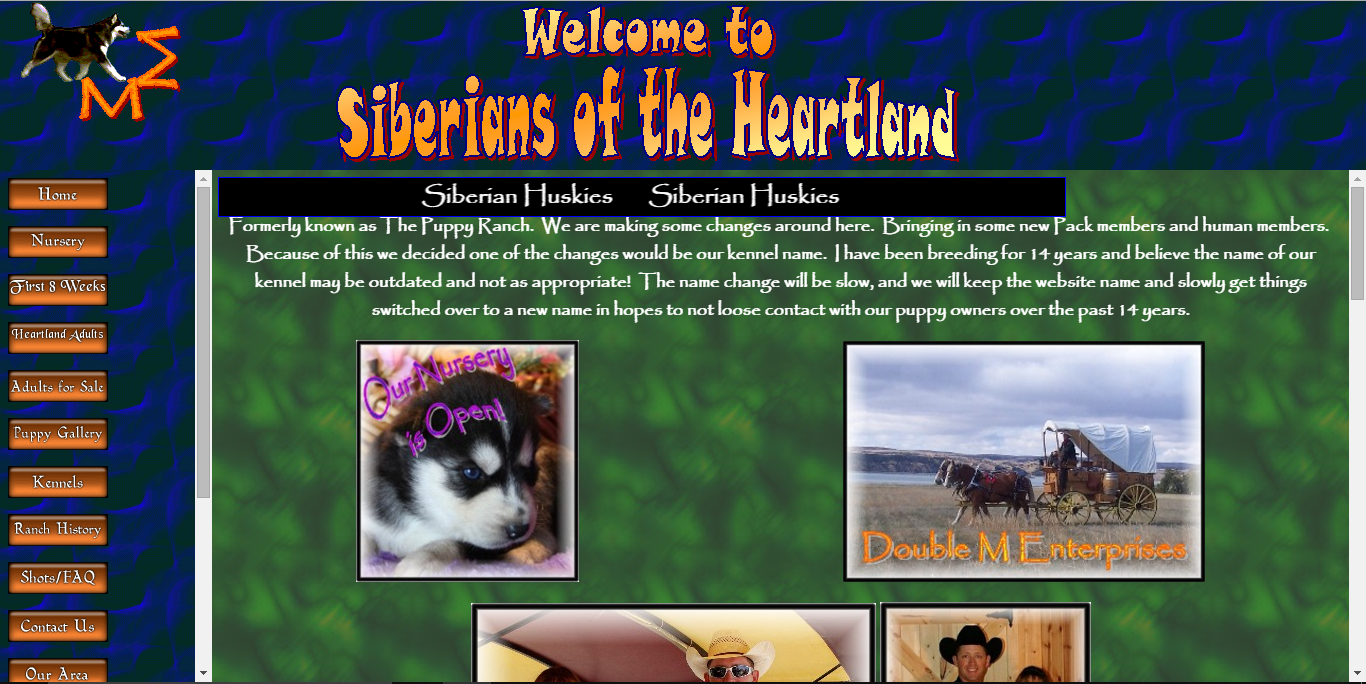
\includegraphics[scale=0.33]{immagini/home.png}
					\caption{La pagina \textit{Home}.}
					\label{fig:home}
		\end{figure}	
		
		\paragraph{Asse \textit{When}}
		Nelle prime righe della pagina vengono riportare le novità riguardo al sito. \textbf{Positivo} ma migliorabile in quanto le novità non si distinguono, a livello visuale, dal resto del testo.
		
		\paragraph{Convenzioni non rispettate}
		
		\begin{figure}[!h]
			\centering
				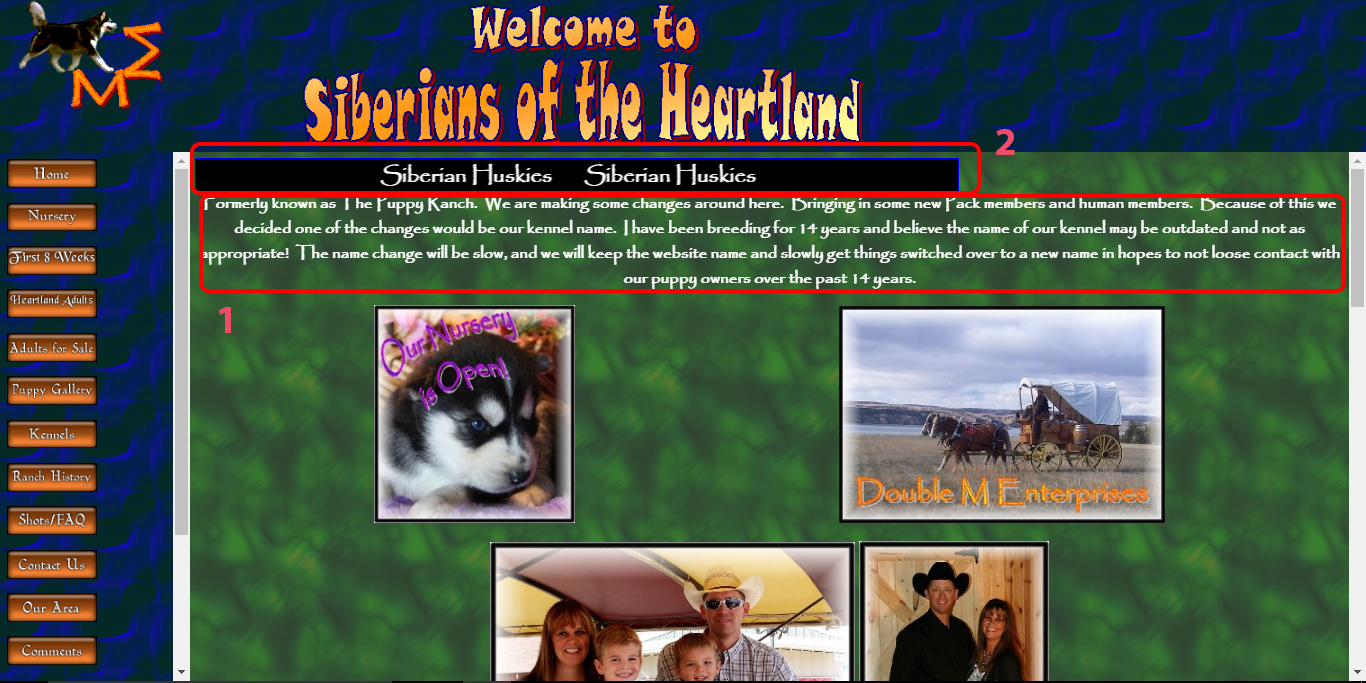
\includegraphics[scale=0.33]{immagini/part_homepage1.jpg}
					\caption{Immagini inconsistenti in \textit{Home}.}
					\label{fig:home1}
		\end{figure}	
		
		\begin{itemize}
	 		\item L'utilizzo delle immagini è inconsistente: alcune sono utilizzate come link mentre altre non sono cliccabili. Ad esempio, le immagini indicate in \hyperref[fig:homefocus]{Figura 1.4} sono dei link cliccabili, mentre le immagini indicate in \hyperref[fig:homefocus]{Figura 1.5} non lo sono. Questo confonde l'utente che scambia i link per immagini e/o viceversa. \textbf{Negativo};
	 		
	 		\item Parti del testo, che non rappresentano link, appaiono sottolineate e/o colorate solo per aumentarne l'enfasi (\hyperref[fig:home1]{Figura 5.1}). L'utente può rimanere frustrato nel provare a cliccare e questo diminuisce il gradimento del sito. \textbf{Negativo}.

	 	\end{itemize}
		
		\paragraph{Bloated design}
		Sotto il titolo della pagina è presente del testo scorrevole che riporta la scritta "Siberian Huskies" (\hyperref[fig:home1]{Figura 5.2}). Questa animazione  rischia di infastidire l'utente. \textbf{Negativo}.		
		
		\newpage
				
\subsubsection{Nursery}
	
		\begin{figure}[!h]
			\centering
				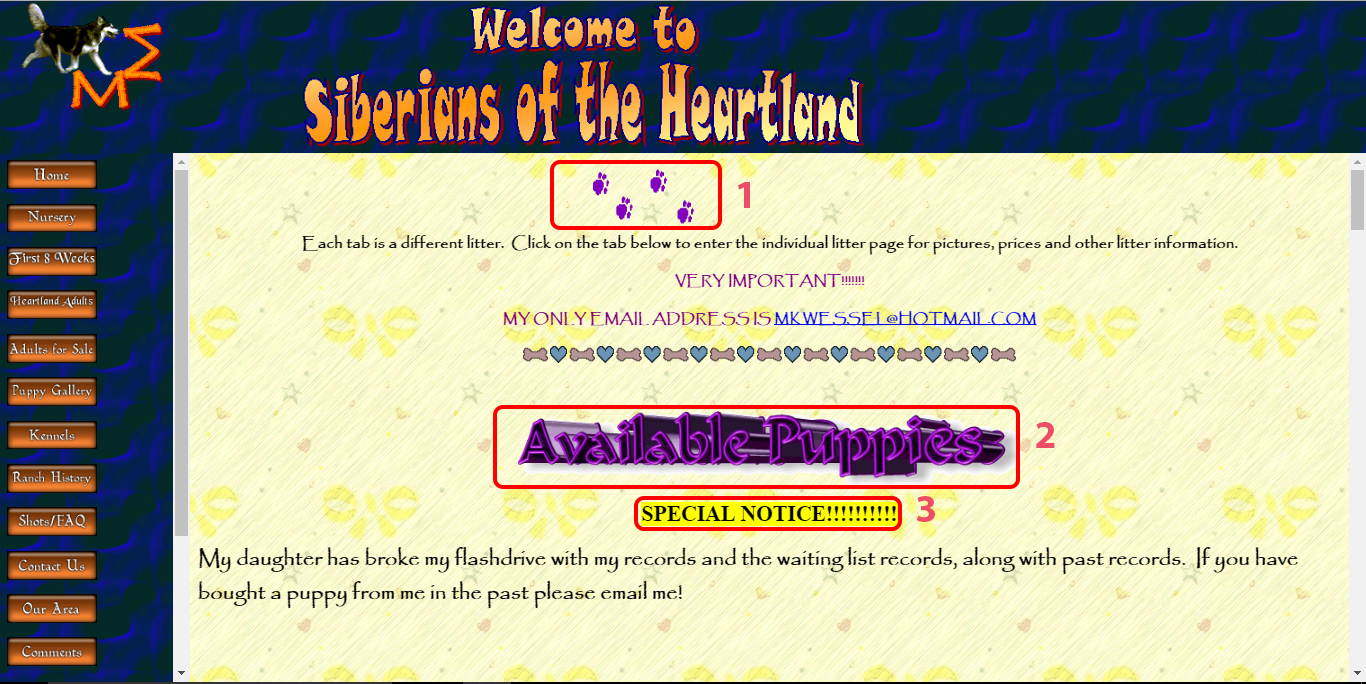
\includegraphics[scale=0.33]{immagini/part_nursery1.jpg}
					\caption{La pagina \textit{Nursery}.}
					\label{fig:nursery1}
		\end{figure}	
	
		\paragraph{Asse \textit{When}}
			Le novità sono divise tra l'inizio della pagina e la fine. Per raggiungere la fine della pagina sono necessari almeno 4 scroll, un nuovo utente non può conoscere questa particolarità mentre un utente che conosce il sito difficilmente sarà portato ad eseguire 4 scroll nella sola speranza di trovare delle \textit{news} interessante. Le novità posizionate a fondo pagina sono quindi praticamente invisibili. \textbf{Negativo}.
		
		\paragraph{Convenzioni non rispettate}
		
		\begin{figure}[!h]
			\centering
				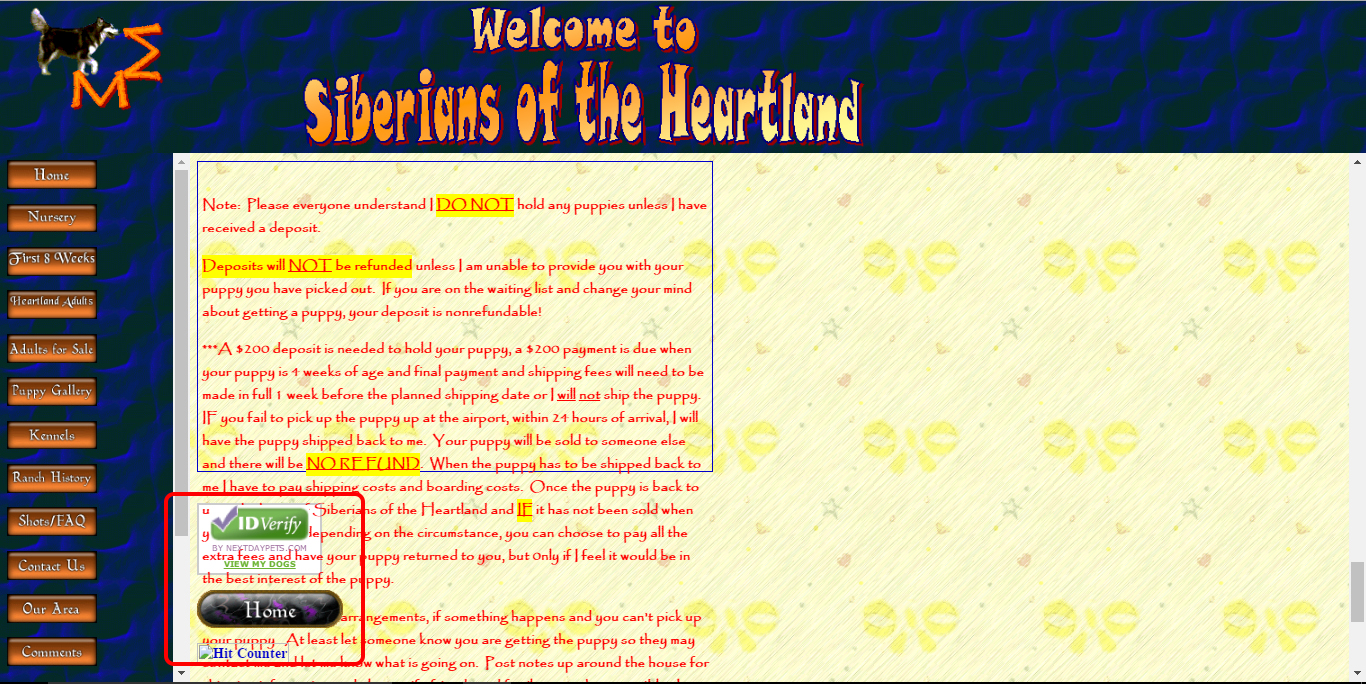
\includegraphics[scale=0.33]{immagini/part_nursery4.jpg}
				\caption{Immagini sovrapposte al testo.}
				\label{fig:nursery4}
			\end{figure}	
		
		\begin{itemize}
	 		\item Dovrebbe essere utilizzato un unico font per il testo dell'intero sito. Solo in questa pagina si possono contare 4 font diversi. \textbf{Negativo};
	 		
	 		\item Per mettere in evidenza alcune parti, il testo è stato inserito come immagine (\hyperref[fig:nursery1]{Figura 6.2}) e questo impedisce all'utente di effettuare le classiche operazioni che ci si aspetta di poter effettuare sul testo. L'utilizzo di testo sotto forma di immagine va inoltre ad appesantire la pagina. \textbf{Negativo};
	 		
	 		\item Testo sottolineato e colorato a solo scopo di enfasi induce l'utente a pensare che sia un link cliccabile o, addirittura, già cliccato (\hyperref[fig:nursery1]{Figura 6.3}). \textbf{Negativo};
	 		
	 		\item I \textit{broken link} sono pericolosi in quando danno false e aspettative all'utente, creando frustrazione. Verso la fine della pagina è presente un bottone che sembra portare alla pagina \textit{Home} (\hyperref[fig:nursery4]{Figura 7}), eventuali click non danno però alcun risultato. \textbf{Negativo}.

	 	\end{itemize}
	 	
	 	\paragraph{Bloated design}
	 	
	 	\begin{figure}[!h]
			\centering
				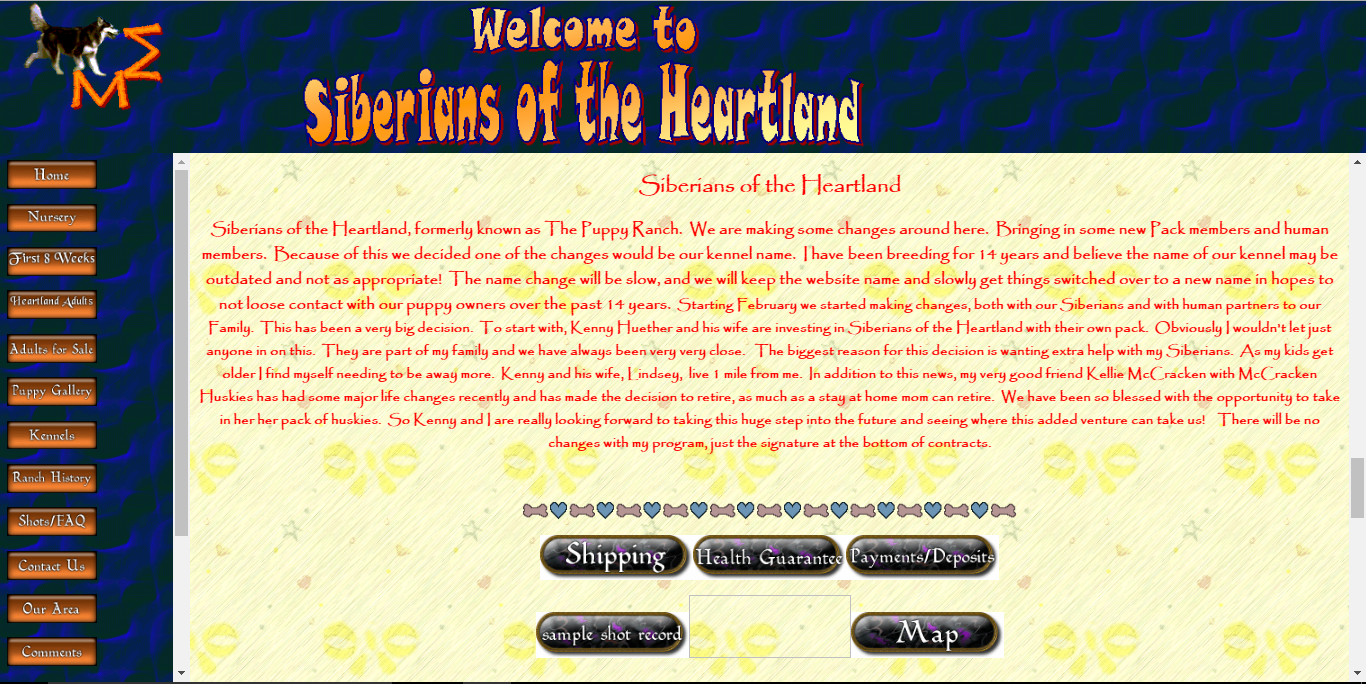
\includegraphics[scale=0.33]{immagini/nursery3.png}
				\caption{Un rettangolo vuoto che funge da link.}
				\label{fig:nursery3}
			\end{figure}	
	 	
	 	\begin{itemize}
	 		\item Sotto il titolo della pagina è presente un'animazione inutile che può affaticare l'occhio del'utente intento nella lettura (\hyperref[fig:nursery1]{Figura 6.1}).  \textbf{Negativo};
	 		
	 		\item Verso metà pagina è presente un rettangolo vuoto che funge da link verso una pagina esterna al sito (\hyperref[fig:nursery3]{Figura 8}). La sua funzione non è per niente intuitiva: l'utente non è portato nè a notarlo nè a cliccarlo. \textbf{Negativo};
	 		
	 		\item Alcune immagini, probabilmente bottoni, sono sovrapposte al testo e lo rendono illeggibile (\hyperref[fig:nursery4]{Figura 7}). \textbf{Negativo}.
	 		
	 	\end{itemize}
			
	\newpage			
			
	\subsubsection{Heartland Adults}
	
	\begin{figure}[!h]
			\centering
				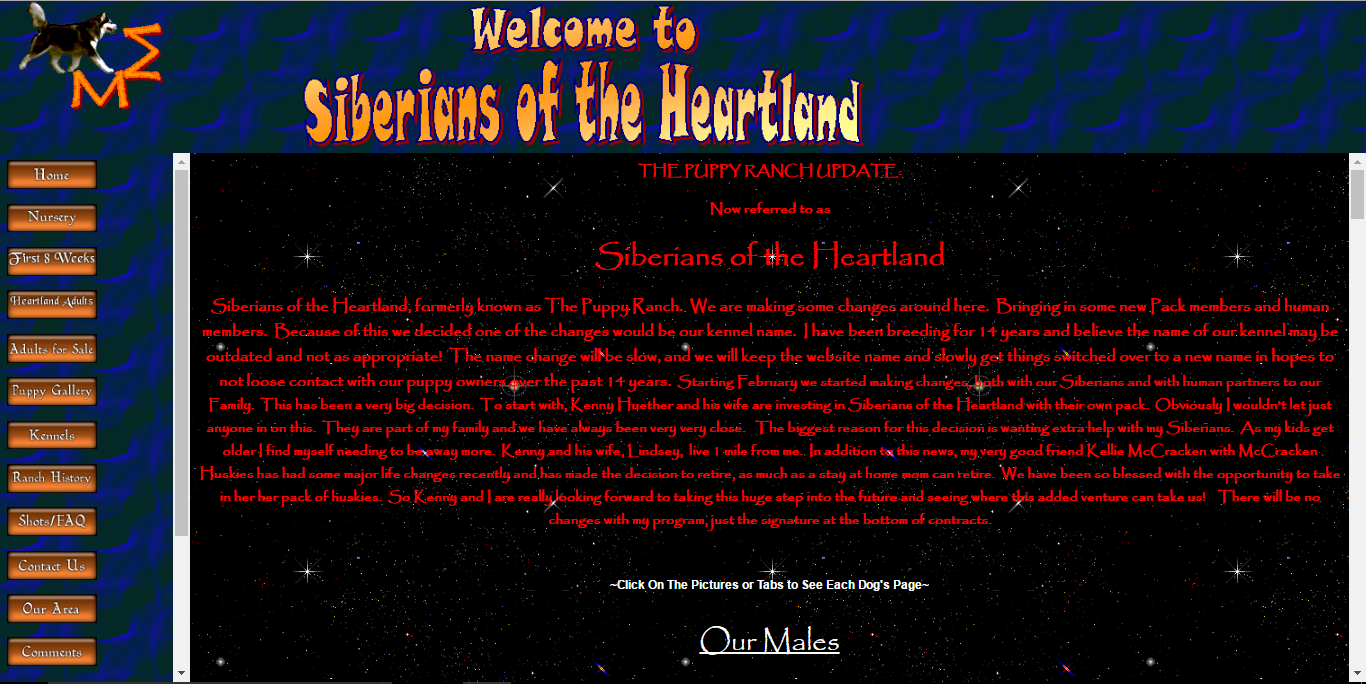
\includegraphics[scale=0.33]{immagini/adults.PNG}
					\caption{La pagina \textit{Heartland Adults}}
					\label{fig:adults}
		\end{figure}	
	
	\paragraph{Asse \textit{When}}
		Nelle prime righe della pagina vengono riportare le novità riguardo al sito. \textbf{Positivo} ma migliorabile in quanto le novità non si distinguono, a livello visuale, dal resto del testo.
	
	\paragraph{Convenzioni non rispettate}
	
		\begin{figure}[!h]
			\centering
				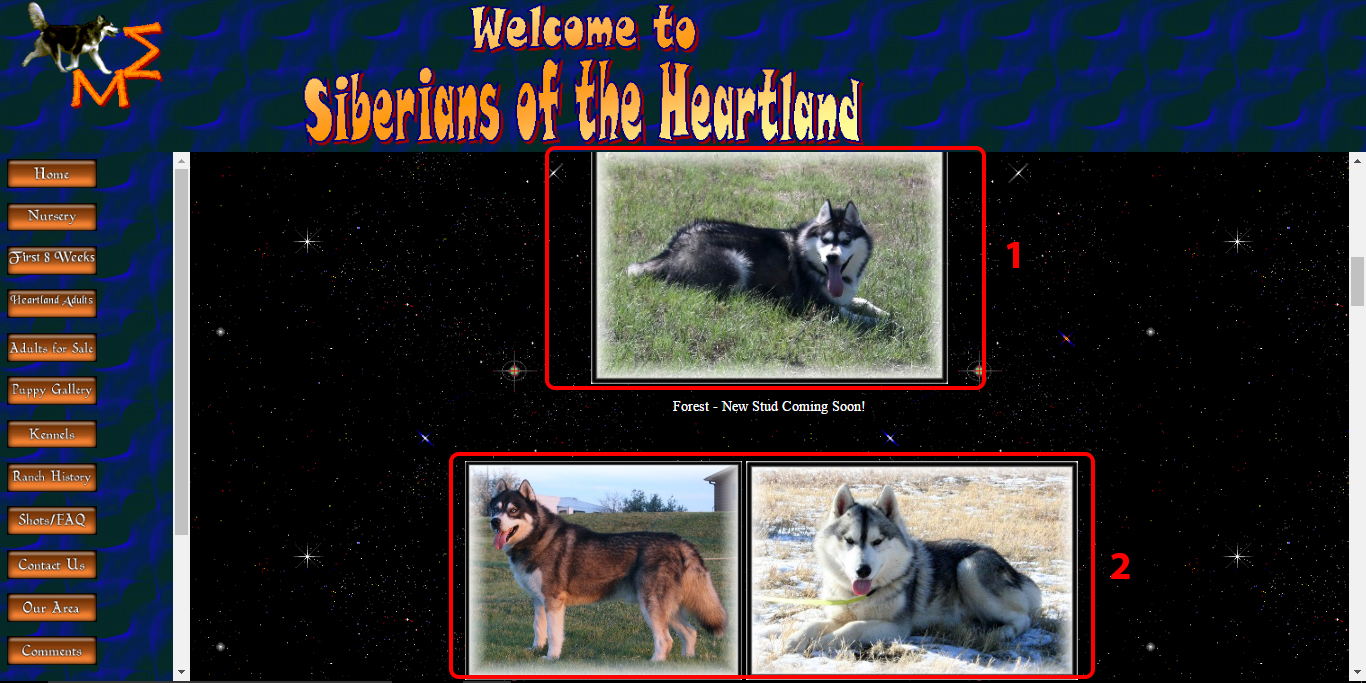
\includegraphics[scale=0.33]{immagini/part_adults1.jpg}
				\caption{Immagini inconsistenti.}
				\label{fig:adults1}
			\end{figure}	
	
	 	\begin{itemize}
	 	
	 		\item L'utilizzo delle immagini è inconsistente: nonostante sia espressamente indicato di "\textit{cliccare sulle immagini per accedere alla pagina dedicata al cane}", alcune immagini sono cliccabili mentre altre no.  Ad esempio, le immagini indicate in \hyperref[fig:adults1]{Figura 10.2} sono dei link cliccabili, mentre l'immagine indicata in \hyperref[fig:adults1]{Figura 10.1} non lo è. Questo crea false speranze nell'utente che non riesce a raggiungere il proprio obiettivo. \textbf{Negativo};
	 		
	 		\item Il testo è sottolineato e colorato a solo scopo di enfasi, questo induce l'utente a pensare che sia un link cliccabile o, addirittura, già cliccato (\hyperref[fig:adults]{Figura 9}). \textbf{Negativo}.
	 	
	 	\end{itemize}
	
	\paragraph{Bloated design}
	Il \textit{background} di questa pagina è caratterizzato da stelle su un fondo nero alle quali è applicato un effetto che le fa "brillare". Se a tale animazione viene abbinato il colore rosso del testo, lo sforzo computazionale necessario alla lettura aumenta di molto. \textbf{Negativo}.
	
\end{document}